\documentclass{article}
\usepackage{xeCJK}
\usepackage{indentfirst}
\usepackage{minted}
\usepackage{fancyhdr}
\pagestyle{fancy}
\usepackage{graphicx}
\usepackage{geometry}
%\geometry{a4paper,centering,scale=0.8}
\usepackage[titletoc]{appendix}
\usepackage[CJKbookmarks=true,colorlinks,linkcolor=black,anchorcolor=blue,citecolor=green]{hyperref}
\usepackage[nottoc]{tocbibind}


\begin{document}
\title{实验报告\\ [2ex] \begin{large}宠物小精灵对战系统 \end{large}}
\author{史柠玮\\
        学号:2014211283\\
        班级:2014211306}
\date{\today}

\maketitle
\tableofcontents

\pagebreak[4]




\section{实验目的}
\label{sec:purpose}
\begin{itemize}
\item 用面向对象的设计方法来来设计一款平台类对战游戏。 
\item 掌握类的继承,对象数据成员设计,成员函数设计.
\item 掌握socket通信,交互场景反馈.
\item 掌握客户端与服务器数据交互(可采用多进程或异步通信或其他方法均可)并发请求处理,类的方法设计,伤害计算方法设计。
\end{itemize}


\section{实验要求}
\label{sec:demand}

\subsection{宠物小精灵的加入}
  \begin{itemize}
  \item 设计宠物小精灵的类,为简化游戏设计,精灵的属性包括种类(力量型:高攻击; 肉盾型:高生命值; 防御型:高防御; 敏捷型:低攻击间隔,共四种)、名字、等级、\emph{*稀有度*}、经验值、攻击力、防御力、生命值、攻击间隔等(要求:本游戏中只有上面的4种类型。 )
  \item 每个精灵初始等级为1,满级15级,每当精灵升级的时候,宠物对应的属性值会有少量增加(主属性增加量相对较多)
  \item 每个精灵有自己独特的攻击方式,如“闪电攻击”,“火焰攻击”等等,请设计一个精灵的基类,并将精灵的攻击方法设为虚方法以方便子类重写
  \item 写一个测试程序对设计的精灵类的相关属性和方法(包括攻击函数,升级函数等)进行测试
  \end{itemize}
\subsection{用户注册与平台登录}
  \begin{itemize}
  \item 每个用户需要注册一个账号,用户名全局唯一,不能有任何两个用户名相同,要考虑注册失败的场景时的反馈
  \item 实现注册、登录、登出功能,均采用C/S模式,客户端和服务端用socket进行通信,服务端保存所有用户的信息(用数据库保存) 
  \item 每个用户拥有属性:用户名、密码、胜场数、总场数。 用户注册成功时,系统自动随机分发三个1级精灵给用户
  \item 用户可以查看所有成功注册用户拥有的精灵,也可以查看所有当前在线的用户
  \item 有界面设计
  \end{itemize}
\subsection{游戏对战的设计}
  \begin{itemize}
  \item 已经登录的在线用户可以和服务器进行虚拟决斗,决斗分两种:升级赛和决斗赛,两种比赛都能增长宠物经验值。服务器上有一个虚拟精灵的列表,用户可以挑选其中任意一个进行比赛(升级赛或者决斗赛)。另外决斗赛中用户胜出可以直接获得该战胜的的精灵,失败则系统从用户的精灵中随机选三个(不够三个精灵的情况就选择他所有的精灵),然后由用户选一个送出。
    \begin{itemize}
    \item 升级赛 只是用户用来增加精灵经验值,规则开发者自定;
    \item 累积多少经验值升一级,规则开发者自定;
    \item 决斗赛的上述规则同升级赛,只是额外还可以赢得宠物一个。
    \end{itemize}
  \item 用户如果没有精灵(比如总是失败,已经全部送出去),则系统会随机放给给他一个初级精灵。
  \item 系统自动模拟每场比赛的每次出招。另外,为了增加不确定性,可以加入概率闪避攻击和暴击伤害机制
    \begin{itemize}
    \item 比赛的过程和结果由系统根据上述规则自动模拟完成,要求结果具有一定的随机性。
    \end{itemize}
  \item 用户增加新功能,可以查看某个用户的胜率
  \item 用户增加新属性,为宠物个数徽章(金银铜)和高级宠物徽章(金银铜),分别根据拥有的宠物个数的多少和拥有高级宠物(15级)个数的多少颁发
  \item 有界面设计
  \end{itemize}


\section{实验环境}
\label{sec:environment}
\begin{itemize}
\item Fedora 25 64位
\item Qt Creator \& Qt 
\item 10.1.19-MariaDB Server
\end{itemize}

\section{概要设计}
\label{sec:brief}

\subsection{宠物小精灵的加入}
  设计一个基类$PokeMon$,有精灵的属性和两个虚函数,分别是升级函数和攻击函数,用于在子类中重写.\\
  生成四个子类分别为
  \begin{itemize}
  \item $PMAgility$
  \item $PMDefense$
  \item $PMShield$
  \item $PMStrength$
  \end{itemize}
  设计不同的稀有倍率常数和类型倍率常数,用于生成精灵时以及升级时相应属性与倍率常数相乘,以体现不同类型和稀有度的区别.
  子类中重写升级函数和构造函数,使用了刚刚定义的倍率常数.\\
  设计8种特殊攻击,每种类型分配两种,每当小精灵被构造,在其两种特殊攻击中随机选择一种赋予.
  测试生成精灵与攻击在GUI上进行, \emph{GUI设计略}\footnote{GUI的设计不属于实验目的,并且描述比较复杂,以下将不涉及GUI设计}

\subsection{用户注册与平台登录}
  \begin{enumerate}
  \item 建立数据库以及建立两张表
    \begin{description}
    \item[users] 包含属性 用户名, MD5加密后的密码
    \item[monsters] 包含属性 名字,拥有者,等级,类型,稀有度,经验值,攻击力,防御力,生命值,攻击间隔,特殊攻击,经验值, id(主键)
    \end{description}
    
\subsubsection{客户端设计}
    使用UDP与服务器进行通信\footnote{服务器与客户端也是使用的UDP,本实验所有通信皆使用的UDP进行通信,以下不再赘述}.\\
    UDP包由包头(自定义$datagramType$类型)和数据构成,例如注册的包由包头($LOGIN$)加上要进行注册的帐号和加密后的密码组成.\footnote{
      全部包的组成请查阅附录\ref{app:udp}.}\\
    客户端发送注册或者登录信息后等待服务器查询数据库并返回确认信息进入主页面,否则报错.
    进入主界面后向服务器发送请求小精灵信息,并等待接收,接收之后显示在主界面上,
    如果用户想要查看其他用户以及小精灵信息,客户端也发送相应的请求包,并等待接收显示.\\
   
  \subsubsection{服务器设计}
    始终监听某一设定好的端口,等待客户端发送请求,读取数据库,并返回相应的信息.
  \end{enumerate}
  
\subsection{游戏对战的设计}
  \begin{enumerate}
  \item 战斗的设计\\
    虚拟计时器(并不真正计时,因此战斗的计算是一瞬间完成的)从0开始计时,按照双方的攻击间隔进行攻击计算,直到有一方生命值归0计时结束,
    并把每次攻击的属性(见附录)\ref{app:movement}(攻击者,伤害,额外伤害,是否暴击,是否闪避,剩余HP等)记录下来,
    进行真正的计时,经过相应时间间隔输出一条,直到输出完毕或者用户点击了跳过,战斗结束,输出战斗结果,并将结果发送至服务器,等待处理,
    如果是决斗赛,进行新小精灵命名或者三选一进行送出,如果是升级赛,则进行经验值获得以及升级.
  \item 对手的选择\\
    用户可以自己设定对手的等级以及稀有度,类型将由服务器随机生成,若战胜则根据不同的稀有度等级倍率常数给予不同的经验值.
  \item 如果服务器检测到有用户精灵全部送出,则随机生成一只一级的给予.
  \item 客户端的徽章由客户端计算,如果超过某个设定的阈值则将其某个特定的徽章设置为相应的.
  \item 数据库中的$users$表增加两个字段,分别为胜场数和总场数,经过客户端请求和服务器应答,胜率将显示在客户端上
  \end{enumerate}
  

\section{详细设计}
\label{sec:detail}

\subsection{宠物小精灵的加入}

  \subsubsection{基类}
  
    \begin{minted}{c++}
  enum PMType
  {
      Strength, Defense, Shield, Agility
  };

  enum PMRarity
  {
      Common, Rare, Epic, Legendary
  };
 
  enum LimitBreak
  {
      FireSpin,//火焰漩涡120\%,灼烧/0
      TakeDown,//猛撞180.,反噬/1
      WaterPulse,//水波动,混乱/2
      PoisonJab,//毒刺,毒/3
      LeechLife,//吸血/4
      Aromatherapy,//芳香治疗,回血,去除异常/5
      AirCutter,//破空斩,暴击/6
      FurySwipes//疯狂乱抓,连续攻击2~5次,/7
      //1⁄6的几率攻击5或4次,1⁄3的几率攻击3或2次,数学期望是3.168次
      OrdAttack//普通攻击
  };

  class PokeMon : public QObject//QObject为Qt规定基类
  {
      Q_OBJECT
  public:
 
      PokeMon();
      PokeMon(PMRarity rarity);
      PokeMon(PokeMon &src);
      ~PokeMon();
      void gainExp(int newExp);//获得经验值,里面会调用levelUp()
      virtual void levelUp();
      virtual int move() = 0;//返回不同攻击所代表的整数
      void rename(QString newName);
      virtual QString getInfomation();
      void setName(QString newName);
  private:
      PMType type;
      PMRarity rarity;
      LimitBreak limitBreak;
      QString name;
      int level;
      int exp;
      double attack;
      double defence;
      double maxHealth;
      double speed;
      int id;
  };
\end{minted}

\subsubsection{其中的一个子类}
注\footnote{其他子类雷同}
  \begin{minted}{c++}
  class PMStrength : public PokeMon
  {
  public:
      PMStrength(PMRarity rarity);//利用稀有度为参数,属性随机生成
      PMStrength(PokeMon& src):PokeMon(src){}
      int move();
      void levelUp();
  };
  \end{minted}

  \subsection{用户注册与平台登录}

  \subsubsection{服务器的接收函数}
    \begin{minted}{c++}
void MainWindow::on_readyRead()
{//这个函数不同时期都有修改添加,所以可能思路有细微改变,导致switch中各个case中读取的方法不统一
    QByteArray datagram;//received datagram
    datagram.resize(server->pendingDatagramSize());
    QHostAddress senderAddr;
    server->readDatagram(datagram.data(),datagram.size(),&senderAddr);
    QString name,word;//sender's name and word
    QDataStream inStream(datagram);
    quint16 port;//port of this client
    datagramType type;//type of this datagram
    inStream>>type;

    QString msg;
    QByteArray msgba;//message to send
    QDataStream outStream(&msgba,QIODevice::ReadWrite);

    switch (type) {
    case LOGIN:
    {
        inStream>>port>>name>>word;
        qDebug()<<port<<name<<word<<"login";
        bool isOk=database->login(name,word);
        if(isOk)
        {
            msg="Yes";
            onLogin(senderAddr,port,name);
        }
        else
            msg="whatever";
        outStream<<msg;
        server->writeDatagram(msgba,senderAddr,port);
    }
        break;
    case SIGNUP:
    {
        inStream>>port>>name>>word;
        qDebug()<<port<<name<<word<<"signup";
        bool isOk=database->signup(name,word);
        if(isOk)
        {
            msg="Yes";
            onSignup(name);
        }
        else
            msg="whatever";
        outStream<<msg;
        server->writeDatagram(msgba,senderAddr,port);
    }
        break;
    case EXIT:
    {
        inStream>>name;
        qDebug()<<name<<"logout";
        onLogout(name);
    }
        break;
    case GETSELFMONS:
    {
        inStream>>name;
        qDebug()<<name<<"GETSELFMONS";
        on_getSelfMons(name);
    }
        break;
    case GETUSERS:
    {
        inStream>>port;
        qDebug()<<port<<"GETUSERS";
        on_getUsers(port,senderAddr);
    }
        break;
    case GETCERTAINMONS:
    {
        inStream>>port>>name;
        qDebug()<<port<<name<<"GETCERTAINMONS";
        on_getCertainMons(port,name,senderAddr);
    }
        break;
    case GETOPPONENT:
    {
        int level;
        int tmpRarity;

        inStream>>port>>name>>level>>tmpRarity;
        qDebug()<<"GETOPPONENT";
        on_getOpponent(port,name,level,(PMRarity)tmpRarity,senderAddr);
        break;
    }
    case SENDRESULT:
    {
        qDebug()<<"SENDRESULT";
        on_sendResult(inStream);
        break;
    }
    case GETTROPHY:
    {
        qDebug()<<name<<"GETTROPHY";
        on_getTrophy(inStream);
        break;
    }
    case KILLPM:
    {
        qDebug()<<"KILLPM";
        on_killPM(inStream);
        break;
    }

    default:
        break;
    }
}
    \end{minted}
  \subsubsection{数据库类的设计}
    \begin{minted}{c++}
class Database
{
public:
    Database();

    QSqlDatabase db;

    bool login(QString username,QString password);

    bool signup(QString username,QString password);

    QStringList allUsers();

    double getWinRate(QString name);

    QList<PokeMon *> pmsOfUser(QString username);

    void addPokeMon(QString owner, PokeMon * pm);

    void updateWinRate(QString name, bool result);

    void deletePokeMon(int id);

    PokeMon *pmAt(int id);

    void updatePM(int id, PokeMon *pm);
};
//简单选取其中一个函数展示
void Database::addPokeMon(QString owner, PokeMon *pm)
{
    QSqlQuery query;
    query.prepare("INSERT INTO monsters (owner, level, type, rarity, attack, defence, maxHealth,"
                  " speed, exp, limitbreak, name) values (?,?,?,?,?,?,?,?,?,?,?)");
    query.addBindValue(QVariant(owner));
    query.addBindValue(QVariant(pm->level));
    query.addBindValue(QVariant((int)pm->type));
    query.addBindValue(QVariant((int)pm->rarity));
    query.addBindValue(QVariant(pm->attack));
    query.addBindValue(QVariant(pm->defence));
    query.addBindValue(QVariant(pm->maxHealth));
    query.addBindValue(QVariant(pm->speed));
    query.addBindValue(QVariant(pm->exp));
    query.addBindValue(QVariant((int)pm->limitBreak));
    query.addBindValue(QVariant(pm->name));
    query.exec();
}

\end{minted}
  
\subsection{游戏对战的设计}

  \subsubsection{战斗函数的设计}
    \begin{minted}{c++}
QList<movement> Fighting::procedure()
{
    QList<movement> procedures;
    int interval_A=SPEEDARG/A->speed;//SPEEDARG=4e6
    int interval_B=SPEEDARG/B->speed;
    int rest_A=interval_A;
    int rest_B=interval_B;
    quint32 time=0;//虚拟计数器
    while(true)
    {
        if(rest_A<rest_B){ // A 攻击
            time+=rest_A;

            int dice=qrand()%100;//随机骰子
            bool critical=false;
            bool miss=false;
            if(dice>90)
                critical=true;//暴击还是闪避?
            else if(dice<10)
                miss=true;

            rest_B-=rest_A;
            rest_A=interval_A;

            LimitBreak move = (LimitBreak)A->move();
            int damage=(A->attack-B->defence)>10?(A->attack-B->defence):10;//计算伤害
            int recovery=0;
            switch (move) {//伤害乘以倍率以及异常状态
            case OrdAttack:
                break;
            case FireSpin:
                damage*=1.5;
                if(!miss)
                  stateA[Burning]=3;
                break;
                //...其他case略
            }

            if(critical)
                damage*=1.5;//暴击闪避倍率
            if(miss)
                damage=0;

            int extraDamage=0;
            if(stateA[Burning])//异常状态额外伤害,以及灼烧降低伤害
            {
                extraDamage=A->maxHealth/10;
                damage*=.7;
            }
            if(stateA[Toxic])
                extraDamage=A->maxHealth/8;
            if(stateA[Confused])
            {
                dice=qrand()%10;
                if(dice<5)
                {
                    extraDamage=damage;
                    damage=0;
                }

            }

            exceptionFade('A');//每次出手所有异常状态回合数减一

            healthPoint_B-=damage;
            healthPoint_A+=(recovery-extraDamage);


            if(healthPoint_A>A->maxHealth)
                healthPoint_A=A->maxHealth;
            else if(healthPoint_A<0)
                healthPoint_A=0;
            if(healthPoint_B<0)
                healthPoint_B=0;
            movement tmp={time, 'A', critical, miss, damage,
                          extraDamage, recovery, move, stateA, stateB,
                          healthPoint_A, healthPoint_B};
            procedures.append(tmp);//保存该条movement
        }
        else //rest_B<rest_A
        {
            //...与上面雷同,略
        }
        if(healthPoint_B==0)
        {
            result=true;
            break;
        }
        else if(healthPoint_A==0)
        {
            result=false;
            break;
        }
    }
    return procedures;
}
\end{minted}
\subsubsection{发送结果数据包(发包举例)}
  \begin{minted}
void Battle::sendResult(int id, bool result, int level, PMRarity rarity)
{
    QByteArray datagram;//datagram to send
    QDataStream outStream(&datagram,QIODevice::ReadWrite);
    datagramType type=SENDRESULT;

    outStream<<type
            <<name
           <<battleType
          <<id
         <<result;

    if(result)//win a race
    {
        int exp = expToGain[level]*((int)rarity+1);
        outStream< <exp;
    }
    else if(battleType==2)   //duel race
    {
        ;//do nothing
    }

    socket->writeDatagram(datagram,serverAddress,serverPort);
}
\end{minted}
发送后等待服务器回应,进行相应操作
\subsubsection{战斗过程展示函数片段}
  \begin{minted}{c++}
auto infos=fight.generateInfo(procs);
ui->label_HPA->setText(QString("%1").arg((int)self->maxHealth));
ui->progressBar_A->setMaximum((int)self->maxHealth);
ui->progressBar_A->setValue((int)self->maxHealth);
ui->label_HPB->setText(QString("%1").arg((int)opponent->maxHealth));
ui->progressBar_B->setMaximum((int)opponent->maxHealth);
ui->progressBar_B->setValue((int)opponent->maxHealth);
QString init=tr("决斗开始:\n你的HP:%1,对方的HP:%2\n").arg(self->maxHealth)
                                  .arg(opponent->maxHealth);
ui->textBrowser_info->append(init);

quint32 preTime=0;
for(int i=0;i<procs.length();i++){

    QElapsedTimer t;//利用Qt库进行特定时间间隔等待,并不会造成未响应状态
    t.start();
    while(t.elapsed()<procs[i].time-preTime&&!isSkipped)
        QCoreApplication::processEvents();

    ui->label_HPA->setText(QString("%1").arg(procs[i].HP_A));
    ui->progressBar_A->setValue(procs[i].HP_A);
    ui->label_HPB->setText(QString("%1").arg(procs[i].HP_B));
    ui->progressBar_B->setValue(procs[i].HP_B);
    ui->textBrowser_info->append(infos[i]);
    preTime=procs[i].time;
}
if(!isSkipped)
    on_pushButton_skip_clicked();

    QMessageBox::information(this,"战斗结果",result?"胜利":"失败");
  \end{minted}
  \subsubsection{其他}
  如获得精灵,送出精灵操作等都可归类于发包通信与数据库操作,与以上已经展示的代码区别比较小,就不再赘述.


\section{实验总结}
\label{sec:summry}
\begin{enumerate}
\item 对于DRY(Don't Repeat Yourself)原则还是实现的不够好,比如战斗函数那里有一大片几乎相同的代码
  ,但是没想到好的方法改进,还需要继续学习.
\item 对于注释有时用中文,有时用英文,造成风格不统一.用中文是想要看起来更清楚,用英文可能是因为不便切换输入法.
\item 解决问题:\\
  \begin{minted}{c++}
    QDataStream &operator>>(QDataStream &in, A *test)
    {
      test=new A;
      in>>test->a;      
      return in;
    }
    
    A *test;
    int i=100;
    QByteArray ba;
    QDataStream outstream(&ba,QIODevice::ReadWrite);
    outstream<<i;
    QDataStream instream(ba);
    instream>>test;
    qDebug()<<test->a;
  \end{minted}
  这段代码执行后输出test->a为0,原因为参数必须为引用,否则无法修改test的值,修改为以下即可
  \begin{minted}{c++}
      QDataStream &operator>>(QDataStream &in, A *&test);
  \end{minted}

\end{enumerate}

\section{用户使用方法}
\label{sec:information}

\subsection{打开服务器端}
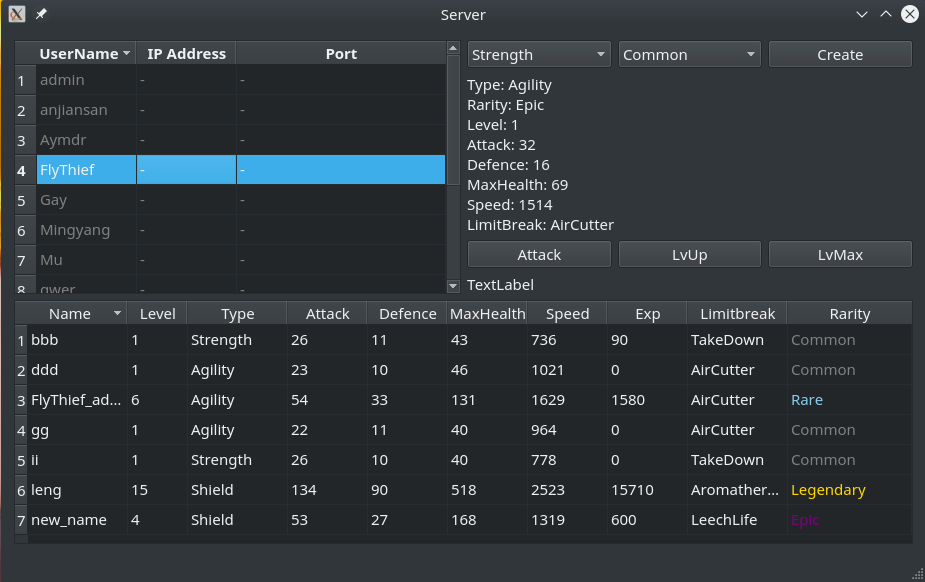
\includegraphics[width=15cm]{./pokemon/服务器.png}

\subsection{注册并登录}

\begin{itemize}
\item 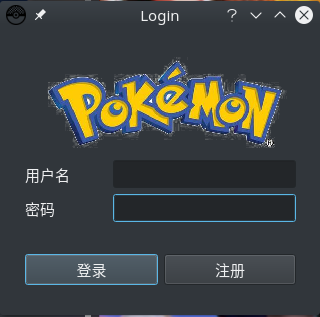
\includegraphics[width=5cm]{./pokemon/登录.png}
\item 点击注册
  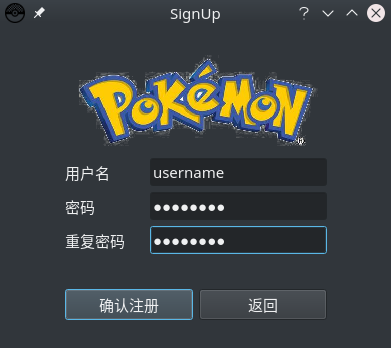
\includegraphics[width=5cm]{./pokemon/注册.png}
\item 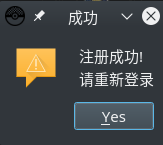
\includegraphics[width=3cm]{./pokemon/注册成功.png}
\item 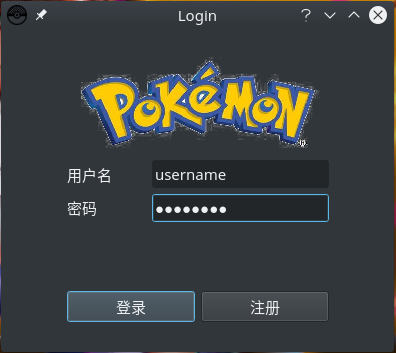
\includegraphics[width=5cm]{./pokemon/登录刚注册的.png}
\end{itemize}



\subsection{客户端主界面}
\begin{itemize}
\item 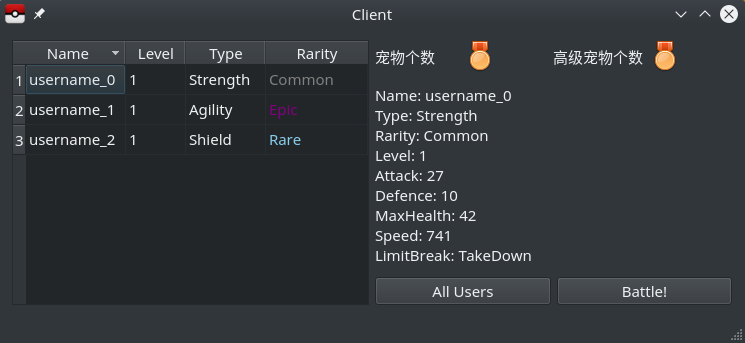
\includegraphics[width=15cm]{./pokemon/客户端主界面.png}
\item 点击All Users\\
  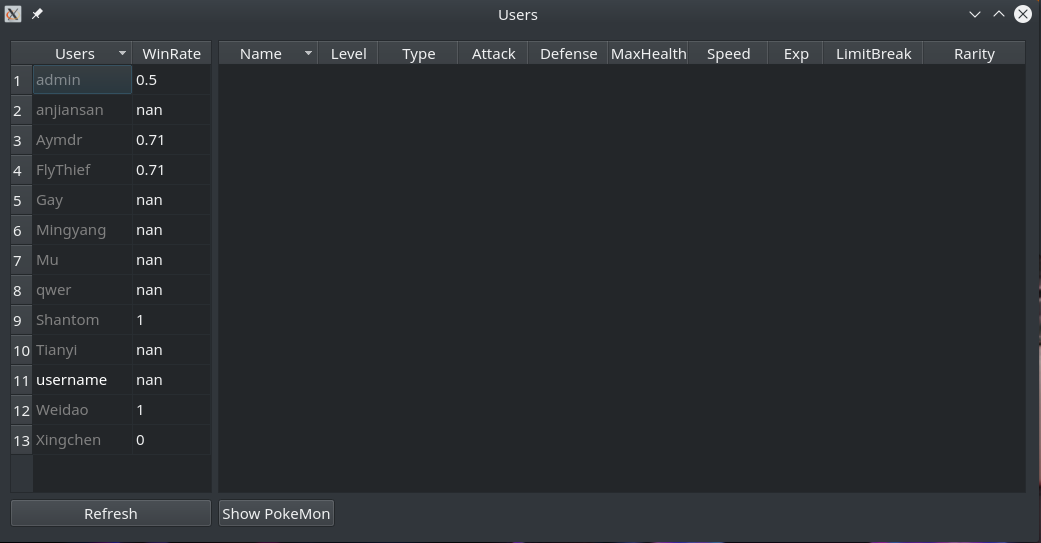
\includegraphics[width=15cm]{./pokemon/查看所有用户.png}
\item 双击某用户\\
  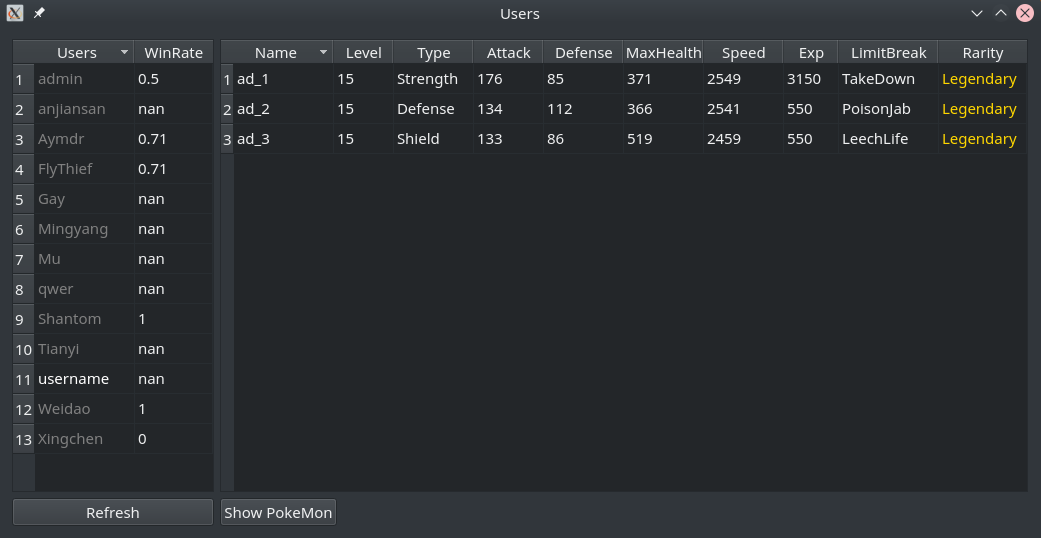
\includegraphics[width=15cm]{./pokemon/查看某用户精灵.png}
\item 返回点击Battle\\
  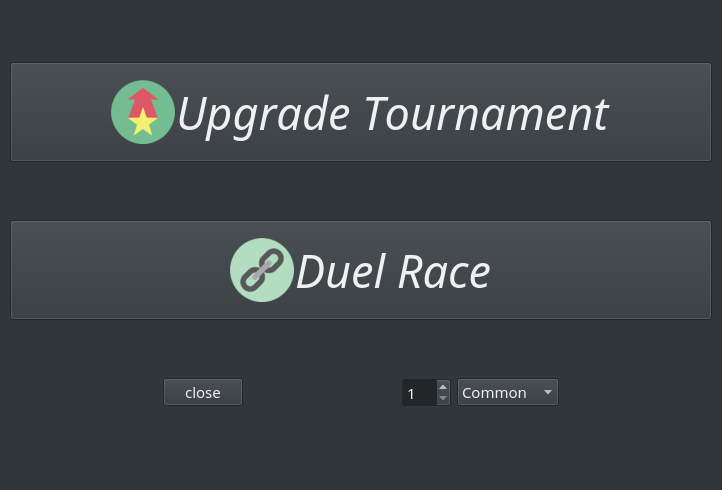
\includegraphics[width=15cm]{./pokemon/战斗选项.png}
  
\end{itemize}

\subsection{战斗画面}
\begin{itemize}
\item 以决斗战为例,点击Battle\\
  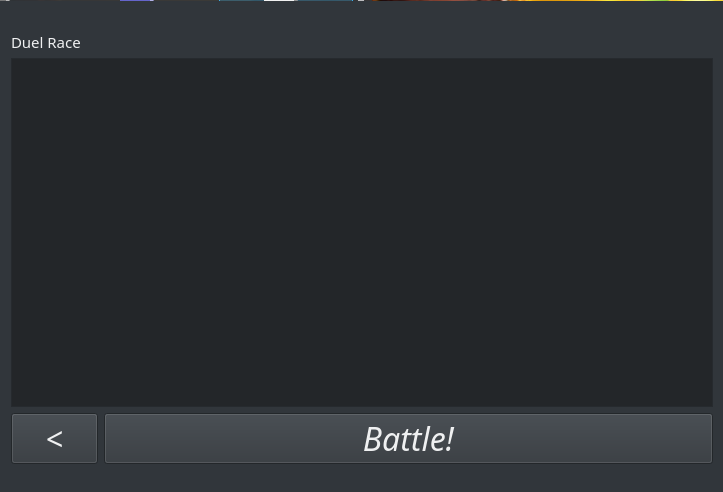
\includegraphics[width=15cm]{./pokemon/Battle.png}
\item 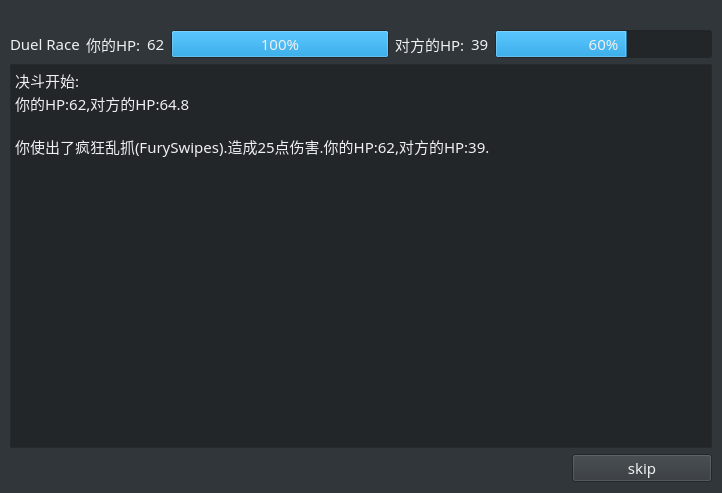
\includegraphics[width=15cm]{./pokemon/战斗过程.png}
\item 点击skip可以跳过,也可等待战斗结束
  \begin{itemize}
  \item 战斗胜利\\
    \begin{center}
    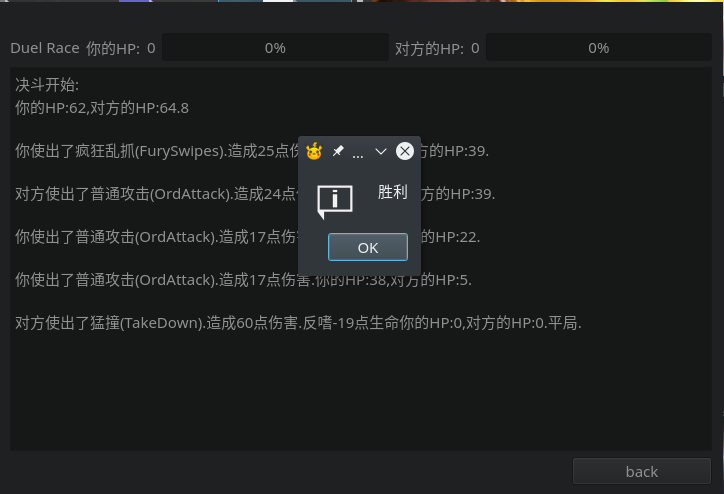
\includegraphics[width=14cm]{./pokemon/战斗胜利.png}
    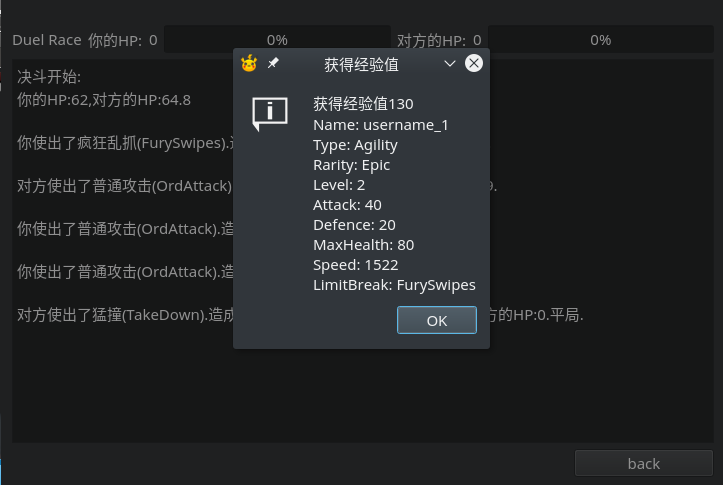
\includegraphics[width=14cm]{./pokemon/获得经验值.png}
    
\includegraphics[width=14cm]{./pokemon/获得小精灵.png}
    可以看到获得了一只新的小精灵\\
    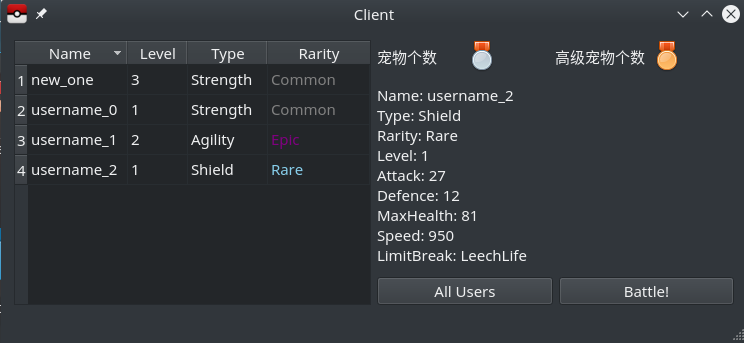
\includegraphics[width=14cm]{./pokemon/获得后.png}
    \end{center}
  \item 战斗失败\\
    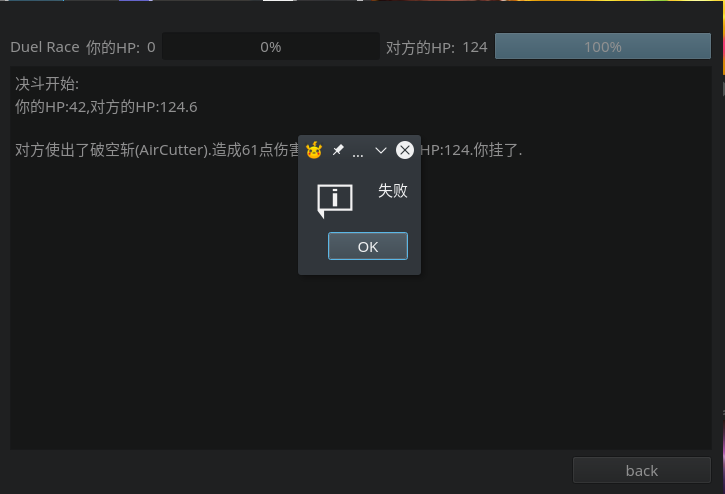
\includegraphics[width=14cm]{./pokemon/战斗失败.png}
    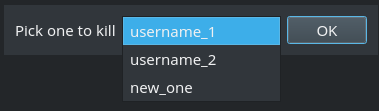
\includegraphics[width=14cm]{./pokemon/送出小精灵.png}
    可以看到送出的小精灵已经消失\\
    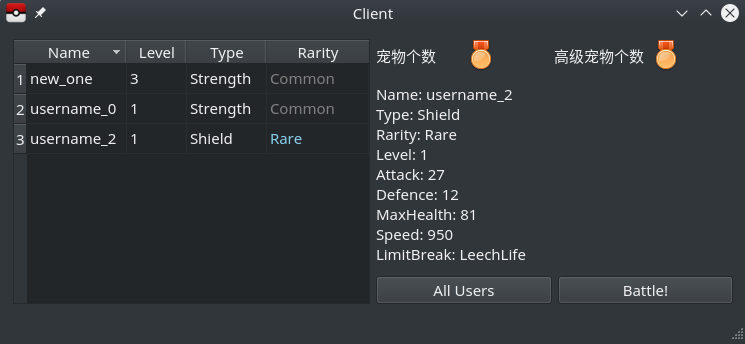
\includegraphics[width=14cm]{./pokemon/送出后.png}
  \end{itemize}
\end{itemize}

\section{附录}
\label{sec:appendix}
本报告中代码的注释有英文也有中文,由本人当时想法不同所致,并非拷贝他人代码,特此声明

\subsection{movement}
\label{app:movement}
\begin{minted}{c++}

  struct movement{
    quint32 time;
    char active;
    bool critical;
    bool miss;
    int damage;
    int extraDamage;
    int recovery;
    LimitBreak method;
    QList<quint8> stateA;
    QList<quint8> stateB;
    qint16 HP_A;
    qint16 HP_B;
};
\end{minted}

\subsection{UDP包结构}
\label{app:udp}
\begin{center}
  \begin{tabular}{|l|l|l|}
    \hline
    头 & 请求包的内容 & 回应包的内容\\ \hline
    LOGIN & port, name, word & ``Yes'' or whatever\\
    SIGNUP & port, name, word & ``Yes'' or whatever\\
    EXIT & name & None\\
    GETSELFMONS & name & allPM(QList<PokeMon*>)\footnote{实际发送的是相应的子类实例}\\
    GETUSERS & port & allUsers(QList<QTableWidgetItem *>\footnote{同样发送的是实例}\\
    GETCERTAINMONS & port, name & allPM\\
    GETOPPONENT & port, name, level, tmpRarity & pm (PokeMon*)\\
    SENDRESULT & name, battleType, id, result & None\\
    KILLPM & id & 1\verb|~|3个pm\\
    GETTROPHY & name, pm & pm\\
   
    \hline
  \end{tabular}
\end{center}

\end{document}






